 \providecommand{\main}{../../..}
\documentclass[\main/main.tex]{subfiles}
\begin{document}
\subsection{Esercizio 2}
Dato il seguente problema di PLI:

\begin{figure}
  \begin{align*}
    \min z = x_2                  \\
    x_1 + x_2  & \leq 5           \\
    -x_1 + x_2 & \leq 0           \\
    \bmx       & \in \mathbb{N}^2
  \end{align*}
  \caption{Esercizio 2}
\end{figure}

\begin{enumerate}
  \item Si ponga in forma canonica rispetto alla base formata dalle variabili $x_1$ e $x_2$ il rilassamento continuo del problema.
  \item Dalla forma canonica si ricavi il taglio di Gomory.
  \item Si disegni la regione ammissibile comprensiva del taglio.
\end{enumerate}

\subsection{Soluzione esercizio 2}
Introduco due variabili di slack $x_3$ e $x_4$:

\begin{align*}
  x_1 + x_2  + x_3 & = 5              \\
  -x_1 + x_2 +x_4  & = 0              \\
  \bmx             & \in \mathbb{N}^4
\end{align*}
Calcolo le matrici in base e fuori base pre moltiplicate
\[
  B = \begin{bmatrix}
    1  & 1 \\
    -1 & 1
  \end{bmatrix}
  \qquad
  B^{-1} = \frac{1}{2}\begin{bmatrix}
    1 & -1 \\
    1 & 1
  \end{bmatrix}
  \qquad
  \bbmb = B^{-1}\bmb = \frac{1}{2}\begin{bmatrix}
    1 & -1 \\
    1 & 1
  \end{bmatrix}
  \begin{bmatrix}
    5 \\
    0
  \end{bmatrix}
  = \frac{5}{2}\begin{bmatrix}
    1 \\
    1
  \end{bmatrix}
  \qquad
  \bar{F} = B^{-1}F = B^{-1}I = B^{-1}
\]
Calcolo i coefficienti di costo ridotti:
\[
  c_0 = -\bmct_B B^{-1} \bmb = - \begin{bmatrix}
    0 & 1
  \end{bmatrix}
  \rnd{
    \frac{1}{2}\begin{bmatrix}
      1 & -1 \\
      1 & 1
    \end{bmatrix}
  }
  \begin{bmatrix}
    5 \\
    0
  \end{bmatrix}
  = - \frac{5}{2}
\]
\[
  \bbmct = \bmct - \bmct_BB^{-1} A =
  \begin{bmatrix}
    0 & 1 & 0 & 0
  \end{bmatrix}
  - \begin{bmatrix}
    0 & 1
  \end{bmatrix}
  \rnd{
    \frac{1}{2}\begin{bmatrix}
      1 & -1 \\
      1 & 1
    \end{bmatrix}
  }
  \begin{bmatrix}
    1  & 1 & 1 & 0 \\
    -1 & 1 & 0 & 1
  \end{bmatrix}
  =\begin{bmatrix}
    0 & 1 & 0 & 0
  \end{bmatrix}
  - \begin{bmatrix}
    0 & 1 & \frac{1}{2} & \frac{1}{2}
  \end{bmatrix}
  = \begin{bmatrix}
    0 & 0 & -\frac{1}{2} & -\frac{1}{2}
  \end{bmatrix}
\]
Ottengo il seguente rilassamento continuo in forma canonica:
\begin{align*}
  \min z = -\frac{5}{2}-\frac{1}{2} x_3 -\frac{1}{2} x_4    \\
  x_1 + \frac{1}{2}x_3 - \frac{1}{2}x_4 & = \frac{5}{2}     \\
  x_2 + \frac{1}{2}x_3 + \frac{1}{2}x_4 & = \frac{5}{2}     \\
  \bmx                                  & \in \R^4_{\geq 0}
\end{align*}

Costruisco il taglio di gomory sul secondo vincolo:

\[
  v_{\text{Gomory}} = (1-\floor{1})x_2 + (\frac{1}{2} - \floor{\frac{2}{2}})x_3 + (\frac{1}{2} - \floor{\frac{1}{2}})x_4 \geq \frac{5}{2} - \floor{\frac{5}{2}} \Rightarrow \frac{1}{2}x_3 + \frac{1}{2}x_4 \geq \frac{1}{2} \Rightarrow x_3 + x_4 \geq 1
\]
Disegno la regione ammissibile sul piano $x_3-x_4$:

\begin{figure}
  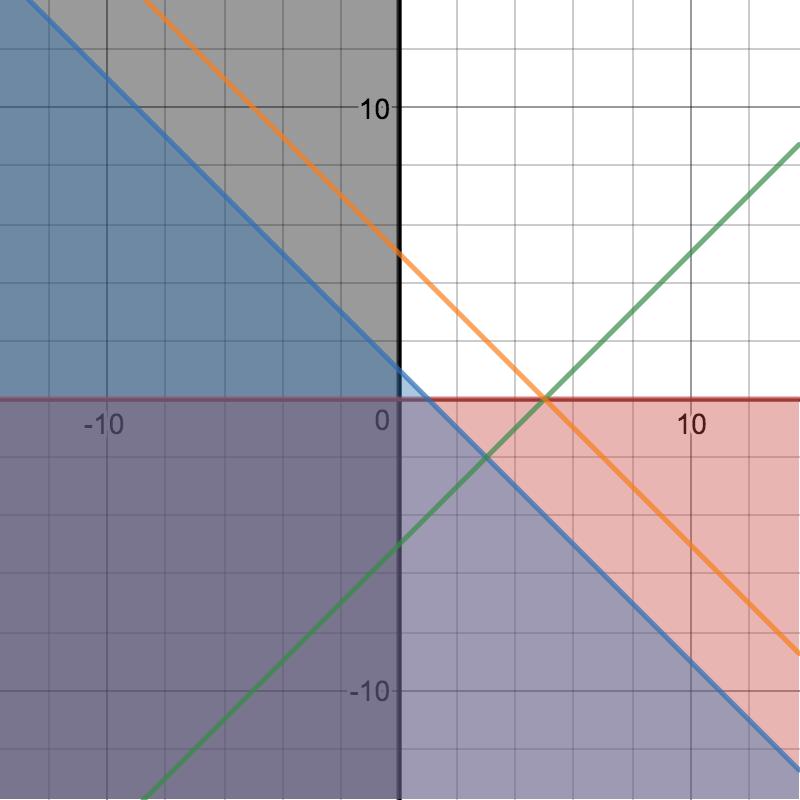
\includegraphics[width=0.4\textwidth]{area_2015_03_gomory}
\end{figure}

\end{document}